\documentclass[10pt]{article}
\usepackage[margin=0.8in]{geometry}
\usepackage[utf8]{inputenc}
\usepackage[T1]{fontenc}
\usepackage{graphicx}
\usepackage[export]{adjustbox}

\usepackage{amsmath}
\usepackage{amsfonts}
\usepackage{amssymb}
\usepackage[version=4]{mhchem}
\usepackage{stmaryrd}
\usepackage{bbold}
\usepackage{fixltx2e}
\usepackage{caption}
\usepackage{mathtools}
\usepackage[parfill]{parskip}
\usepackage{float}

\begin{document}



\title{Lecture 11-12: Jacobian}
\date{Sep. 21, 2023 \quad Sep. 26. 2023 }
\author{Wanxin Jin}
\maketitle


The kinematics equation of  an $n$-DOF manipulator is

$$
\boldsymbol{T}_{e}(\boldsymbol{q})=\left[\begin{array}{cc}
\boldsymbol{R}_{e}(\boldsymbol{q}) & \boldsymbol{p}_{e}(\boldsymbol{q}) \\
\mathbf{0}^{T} & 1
\end{array}\right]
$$

where $\boldsymbol{q}=\left[q_{1},\ldots, q_{n}\right]^{T}$. The goal of the differential kinematics is to find the relationship between the joint velocities and the end-effector linear and angular velocities. In other words, we want to find end-effector linear velocity $\dot{\boldsymbol{p}}_{e}$ and angular velocity $\boldsymbol{\omega}_{e}$ as a function of the joint velocities $\dot{\boldsymbol{q}}$.

$$
\begin{aligned}
& \dot{\boldsymbol{p}}_{e}=\boldsymbol{J}_{P}(\boldsymbol{q}) \dot{\boldsymbol{q}} \\
& \boldsymbol{\omega}_{e}=\boldsymbol{J}_{O}(\boldsymbol{q}) \dot{\boldsymbol{q}}
\end{aligned}
$$

In compact form, the above will be written as

$$
\boldsymbol{v}_{e}=\left[\begin{array}{c}
\dot{\boldsymbol{p}}_{e} \\
\boldsymbol{\omega}_{e}
\end{array}\right]=\boldsymbol{J}(\boldsymbol{q}) \dot{\boldsymbol{q}}
$$

The $(6 \times n)$ matrix $\boldsymbol{J}(\boldsymbol{q})$ is the  geometric Jacobian

$$
    \boldsymbol{J}(\boldsymbol{q})=\left[\begin{array}{l}
\boldsymbol{J}_{P}(\boldsymbol{q}) \\
\boldsymbol{J}_{O}(\boldsymbol{q})
\end{array}\right]
$$

where $\boldsymbol{J}_{P}(\boldsymbol{q})$ is called linear Jacobian and $\boldsymbol{J}_{O}(\boldsymbol{q})$ angular Jacobian.


\section{Linear Jacobian}

To compute linear Jacobian $\boldsymbol{J}_{P}(\boldsymbol{q})$, we can write the time derivative of $\boldsymbol{p}_{e}$ as

$$
\dot{\boldsymbol{p}}_{e}=\boldsymbol{J}_{P} \dot{\boldsymbol{q}}=\sum_{i=1}^{n} \boldsymbol{J}_{P i} \dot{q}_{i} .
$$


This expression shows how $\dot{\boldsymbol{p}}_{e}$ can be obtained as the sum of the terms $\dot{q}_{i} \boldsymbol{J}_{P i}$ Each term represents the contribution of the velocity of single Joint $i$ to the end-effector linear velocity when all the other joints are still.





If Joint $i$ is prismatic, 
  
  $$
\dot{q}_{i} \boldsymbol{J}_{P i}=\dot{d}_{i} \boldsymbol{z}_{i-1}
$$

and then

$$
\boldsymbol{J}_{P i}=\boldsymbol{z}_{i-1} \text {. }
$$

If Joint $i$ is revolute, 


$$
\dot{q}_{i} \boldsymbol{J}_{P i}=\boldsymbol{\omega}_{i-1, i} \times \boldsymbol{r}_{i-1, e}=\dot{\vartheta}_{i} \boldsymbol{z}_{i-1} \times\left(\boldsymbol{p}_{e}-\boldsymbol{p}_{i-1}\right)
$$

and then

$$
\boldsymbol{J}_{P i}=\boldsymbol{z}_{i-1} \times\left(\boldsymbol{p}_{e}-\boldsymbol{p}_{i-1}\right)
$$




\section{Angular Jacobian}


To compute angular Jacobian $\boldsymbol{J}_{O}(\boldsymbol{q})$



$$
\boldsymbol{\omega}_{e}=\sum_{i=1}^{n} \boldsymbol{\omega}_{i-1, i}=\sum_{i=1}^{n} \boldsymbol{J}_{O i} \dot{q}_{i}
$$

 If Joint $i$ is prismatic, it is

  $$
\dot{q}_{i} \boldsymbol{J}_{O i}=\mathbf{0}
$$

and then

$$
\boldsymbol{J}_{O i}=\mathbf{0}
$$

If Joint $i$ is revolute, it is

 $$
\dot{q}_{i} \boldsymbol{J}_{O i}=\dot{\vartheta}_{i} \boldsymbol{z}_{i-1}
$$

and then

$$
\boldsymbol{J}_{O i}=\boldsymbol{z}_{i-1}
$$

\section{Summary}





In summary, the Jacobian can be partitioned into the $(3 \times 1)$ column vectors $\boldsymbol{J}_{P i}$ and $\boldsymbol{J}_{O i}$ as

$$
\boldsymbol{J}=\left[\begin{array}{lll}
\boldsymbol{J}_{P 1} & & \boldsymbol{J}_{P n} \\
& \cdots & \\
\boldsymbol{J}_{O 1} & & \boldsymbol{J}_{O n}
\end{array}\right]
$$

where

\begin{equation} \label{c2.l1.equ5}
    \left[\begin{array}{l}
\boldsymbol{J}_{P i} \\
\boldsymbol{J}_{O i}
\end{array}\right]= \begin{cases}{\left[\begin{array}{c}
\boldsymbol{z}_{i-1} \\
\mathbf{0}
\end{array}\right]} & \text { for a prismatic joint } \\[14pt]
{\left[\begin{array}{cc}
\boldsymbol{z}_{i-1} \times\left(\boldsymbol{p}_{e}-\boldsymbol{p}_{i-1}\right) \\
\boldsymbol{z}_{i-1}
\end{array}\right]} & \text { for a revolute joint. }\end{cases}
\end{equation}

The above allow Jacobian computation in a simple, systematic way on the basis of direct kinematics relations. In fact, the vectors $\boldsymbol{z}_{i-1}, \boldsymbol{p}_{e}$ and $\boldsymbol{p}_{i-1}$ are all functions of the joint variables. 

In particular,
$\boldsymbol{z}_{i-1}$ is given by the third column of the rotation matrix $\boldsymbol{R}_{i-1}^{0}$, i.e.,
  $$
\boldsymbol{z}_{i-1}=\boldsymbol{R}_{1}^{0}\left(q_{1}\right) \ldots \boldsymbol{R}_{i-1}^{i-2}\left(q_{i-1}\right) \boldsymbol{z}_{0}
$$

where $\boldsymbol{z}_{0}=\left[\begin{array}{lll}0 & 0 & 1\end{array}\right]^{T}$ allows the selection of the third column. $\boldsymbol{p}_{e}$ is the first three elements of the fourth column of the transformation matrix $\boldsymbol{T}_{e}^{0}$, i.e., by expressing $\widetilde{\boldsymbol{p}}_{e}$ in the $(4 \times 1)$ homogeneous form

  $$
\widetilde{\boldsymbol{p}}_{e}=\boldsymbol{A}_{1}^{0}\left(q_{1}\right) \ldots \boldsymbol{A}_{n}^{n-1}\left(q_{n}\right) \widetilde{\boldsymbol{p}}_{0}
$$

where $\widetilde{\boldsymbol{p}}_{0}=\left[\begin{array}{llll}0 & 0 & 0 & 1\end{array}\right]^{T}$ allows the selection of the fourth column.  $\boldsymbol{p}_{i-1}$ is  the first three elements of the fourth column of the transformation matrix $\boldsymbol{T}_{i-1}^{0}$, 

$$
\widetilde{\boldsymbol{p}}_{i-1}=\boldsymbol{A}_{1}^{0}\left(q_{1}\right) \ldots \boldsymbol{A}_{i-1}^{i-2}\left(q_{i-1}\right) \widetilde{\boldsymbol{p}}_{0} .
$$





\section{Examples}

\subsection{Three-link Planar Arm}



\begin{figure}[H]
    \centering
   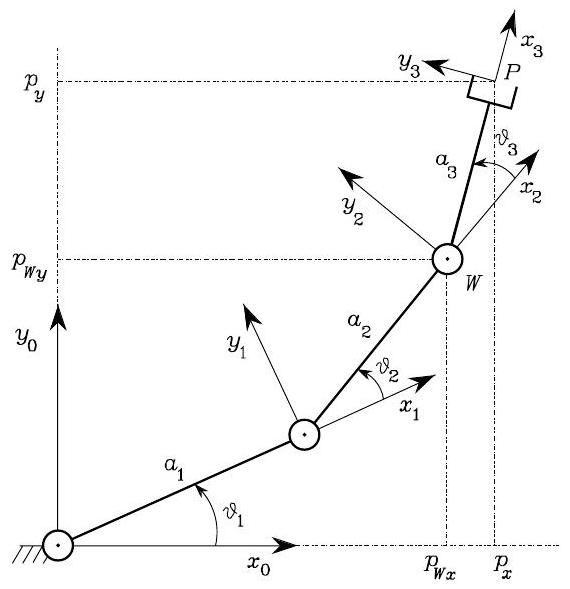
\includegraphics[max width=0.35\textwidth]{./kinematics/3link_arm}
    \label{c1.l2.three-link-robot-arm}
\end{figure}



The Jacobian is

$$
\boldsymbol{J}(\boldsymbol{q})=\left[\begin{array}{ccc}
\boldsymbol{z}_{0} \times\left(\boldsymbol{p}_{3}-\boldsymbol{p}_{0}\right) & \boldsymbol{z}_{1} \times\left(\boldsymbol{p}_{3}-\boldsymbol{p}_{1}\right) & \boldsymbol{z}_{2} \times\left(\boldsymbol{p}_{3}-\boldsymbol{p}_{2}\right) \\
\boldsymbol{z}_{0} & \boldsymbol{z}_{1} & \boldsymbol{z}_{2}
\end{array}\right]
$$

Computation of the position vectors of the various links gives

$$
\boldsymbol{p}_{0}=\left[\begin{array}{l}
0 \\
0 \\
0
\end{array}\right] \quad \boldsymbol{p}_{1}=\left[\begin{array}{c}
a_{1} c_{1} \\
a_{1} s_{1} \\
0
\end{array}\right] \quad \boldsymbol{p}_{2}=\left[\begin{array}{c}
a_{1} c_{1}+a_{2} c_{12} \\
a_{1} s_{1}+a_{2} s_{12} \\
0
\end{array}\right]
\quad
\boldsymbol{p}_{3}=\left[\begin{array}{c}
a_{1} c_{1}+a_{2} c_{12}+a_{3} c_{123} \\
a_{1} s_{1}+a_{2} s_{12}+a_{3} s_{123} \\
0
\end{array}\right]
$$


while computation of the unit vectors of revolute joint axes gives

$$
\boldsymbol{z}_{0}=\boldsymbol{z}_{1}=\boldsymbol{z}_{2}=\left[\begin{array}{l}
0 \\
0 \\
1
\end{array}\right]
$$

since they are all parallel to axis $z_{0}$. Then,
$$
\boldsymbol{J}=\left[\begin{array}{ccc}
-a_{1} s_{1}-a_{2} s_{12}-a_{3} s_{123} & -a_{2} s_{12}-a_{3} s_{123} & -a_{3} s_{123} \\
a_{1} c_{1}+a_{2} c_{12}+a_{3} c_{123} & a_{2} c_{12}+a_{3} c_{123} & a_{3} c_{123} \\
0 & 0 & 0 \\
0 & 0 & 0 \\
0 & 0 & 0 \\
1 & 1 & 1
\end{array}\right]
$$



\subsection{Anthropomorphic Arm}


\begin{figure}[H]
    \centering
   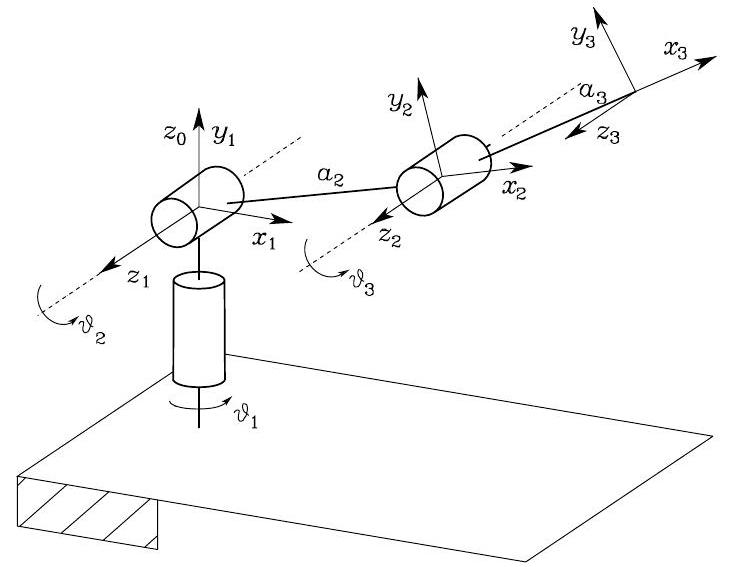
\includegraphics[max width=0.4\textwidth]{./kinematics/anthropomorphic_arm}
\end{figure}


The Jacobian is

$$
\boldsymbol{J}=\left[\begin{array}{ccc}
\boldsymbol{z}_{0} \times\left(\boldsymbol{p}_{3}-\boldsymbol{p}_{0}\right) & \boldsymbol{z}_{1} \times\left(\boldsymbol{p}_{3}-\boldsymbol{p}_{1}\right) & \boldsymbol{z}_{2} \times\left(\boldsymbol{p}_{3}-\boldsymbol{p}_{2}\right) \\
\boldsymbol{z}_{0} & \boldsymbol{z}_{1} & \boldsymbol{z}_{2}
\end{array}\right]
$$

Computation of the position vectors of the various links gives

$$
\begin{gathered}
\boldsymbol{p}_{0}=\boldsymbol{p}_{1}=\left[\begin{array}{l}
0 \\
0 \\
0
\end{array}\right] \quad \boldsymbol{p}_{2}=\left[\begin{array}{c}
a_{2} c_{1} c_{2} \\
a_{2} s_{1} c_{2} \\
a_{2} s_{2}
\end{array}\right] \quad
\boldsymbol{p}_{3}=\left[\begin{array}{c}
c_{1}\left(a_{2} c_{2}+a_{3} c_{23}\right) \\
s_{1}\left(a_{2} c_{2}+a_{3} c_{23}\right) \\
a_{2} s_{2}+a_{3} s_{23}
\end{array}\right]
\end{gathered}
$$

while computation of the unit vectors of revolute joint axes gives

$$
\boldsymbol{z}_{0}=\left[\begin{array}{l}
0 \\
0 \\
1
\end{array}\right] \quad \boldsymbol{z}_{1}=\boldsymbol{z}_{2}=\left[\begin{array}{c}
s_{1} \\
-c_{1} \\
0
\end{array}\right]
$$

Then,

$$
\boldsymbol{J}=\left[\begin{array}{ccc}
-s_{1}\left(a_{2} c_{2}+a_{3} c_{23}\right) & -c_{1}\left(a_{2} s_{2}+a_{3} s_{23}\right) & -a_{3} c_{1} s_{23} \\
c_{1}\left(a_{2} c_{2}+a_{3} c_{23}\right) & -s_{1}\left(a_{2} s_{2}+a_{3} s_{23}\right) & -a_{3} s_{1} s_{23} \\
0 & a_{2} c_{2}+a_{3} c_{23} & a_{3} c_{23} \\
0 & s_{1} & s_{1} \\
0 & -c_{1} & -c_{1} \\
1 & 0 & 0
\end{array}\right]
$$



\subsection{Stanford Manipulator}


\begin{figure}[H]
    \centering
    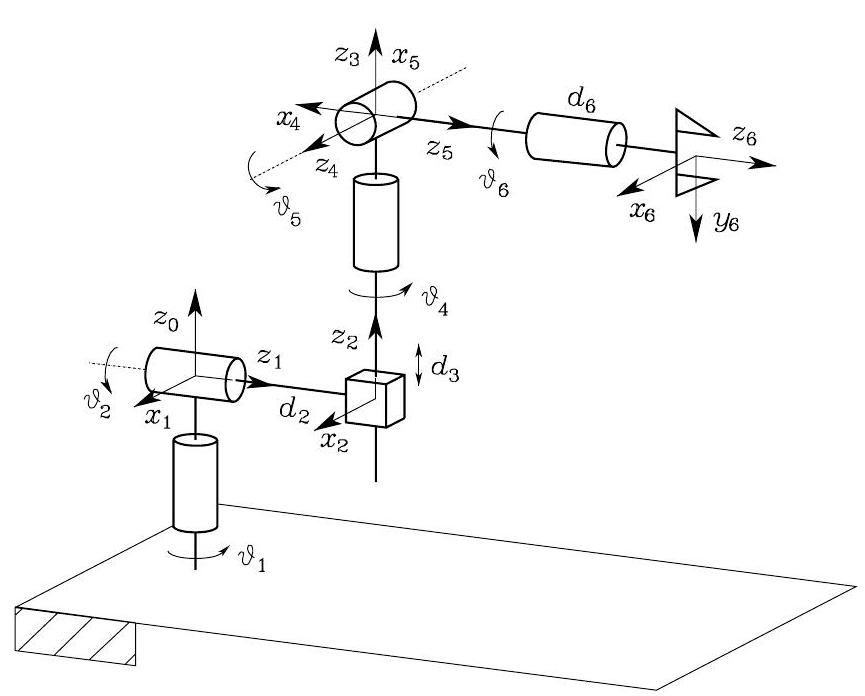
\includegraphics[max width=0.45\textwidth]{./kinematics/Stanford_manipulator}
    \label{c1.l2.fig.Stanford}
\end{figure}


The Jacobian

$$
\boldsymbol{J}=\left[\begin{array}{cccccc}
\boldsymbol{z}_{0} \times\left(\boldsymbol{p}_{6}-\boldsymbol{p}_{0}\right) & \boldsymbol{z}_{1} \times\left(\boldsymbol{p}_{6}-\boldsymbol{p}_{1}\right) & \boldsymbol{z}_{2} &
\boldsymbol{z}_{3} \times\left(\boldsymbol{p}_{6}-\boldsymbol{p}_{3}\right) & \boldsymbol{z}_{4} \times\left(\boldsymbol{p}_{6}-\boldsymbol{p}_{4}\right) & \boldsymbol{z}_{5} \times\left(\boldsymbol{p}_{6}-\boldsymbol{p}_{5}\right)\\
\boldsymbol{z}_{0} & \boldsymbol{z}_{1} & \mathbf{0} & \boldsymbol{z}_{3} & \boldsymbol{z}_{4} & \boldsymbol{z}_{5} \\
\end{array}\right] .
$$

Computation of the position vectors of the various links gives

$$
\begin{gathered}
\boldsymbol{p}_{0}=\boldsymbol{p}_{1}=\left[\begin{array}{l}
0 \\
0 \\
0
\end{array}\right] \quad \boldsymbol{p}_{3}=\boldsymbol{p}_{4}=\boldsymbol{p}_{5}=\left[\begin{array}{c}
c_{1} s_{2} d_{3}-s_{1} d_{2} \\
s_{1} s_{2} d_{3}+c_{1} d_{2} \\
c_{2} d_{3}
\end{array}\right] \quad
\boldsymbol{p}_{6}=\left[\begin{array}{c}
c_{1} s_{2} d_{3}-s_{1} d_{2}+\left(c_{1}\left(c_{2} c_{4} s_{5}+s_{2} c_{5}\right)-s_{1} s_{4} s_{5}\right) d_{6} \\
s_{1} s_{2} d_{3}+c_{1} d_{2}+\left(s_{1}\left(c_{2} c_{4} s_{5}+s_{2} c_{5}\right)+c_{1} s_{4} s_{5}\right) d_{6} \\
c_{2} d_{3}+\left(-s_{2} c_{4} s_{5}+c_{2} c_{5}\right) d_{6}
\end{array}\right],
\end{gathered}
$$

while computation of the unit vectors of joint axes gives

$$
\begin{gathered}
\boldsymbol{z}_{0}=\left[\begin{array}{l}
0 \\
0 \\
1
\end{array}\right] \quad \boldsymbol{z}_{1}=\left[\begin{array}{c}
-s_{1} \\
c_{1} \\
0
\end{array}\right] \quad \boldsymbol{z}_{2}=\boldsymbol{z}_{3}=\left[\begin{array}{c}
c_{1} s_{2} \\
s_{1} s_{2} \\
c_{2}
\end{array}\right] \\
\boldsymbol{z}_{4}=\left[\begin{array}{c}
-c_{1} c_{2} s_{4}-s_{1} c_{4} \\
-s_{1} c_{2} s_{4}+c_{1} c_{4} \\
s_{2} s_{4}
\end{array}\right] \quad \boldsymbol{z}_{5}=\left[\begin{array}{c}
c_{1}\left(c_{2} c_{4} s_{5}+s_{2} c_{5}\right)-s_{1} s_{4} s_{5} \\
s_{1}\left(c_{2} c_{4} s_{5}+s_{2} c_{5}\right)+c_{1} s_{4} s_{5} \\
-s_{2} c_{4} s_{5}+c_{2} c_{5}
\end{array}\right] .
\end{gathered}
$$




\section{Analytical Jacobian}
The  geometric Jacobian is a mapping from  joint velocities to the end-effector linear and angular velocity

$$
    \boldsymbol{v}_{e}=\left[\begin{array}{c}
\dot{\boldsymbol{p}}_{e} \\
\boldsymbol{\omega}_{e}
\end{array}\right]=\boldsymbol{J}(\boldsymbol{q}) \dot{\boldsymbol{q}}
$$


If the end-effector pose is specified in terms of a minimal number of parameters in the operational space, say

$$
{\boldsymbol{x}}_{e}=\left[\begin{array}{c}
{\boldsymbol{p}}_{e} \\
{\boldsymbol{\phi}}_{e}
\end{array}\right]
$$

we need to find a Jacobian in terms of

$$
    \dot{\boldsymbol{x}}_{e}=\left[\begin{array}{c}
\dot{\boldsymbol{p}}_{e} \\
\dot{\boldsymbol{\phi}}_{e}
\end{array}\right]=\boldsymbol{J}_{A}(\boldsymbol{q}) \dot{\boldsymbol{q}}$$

which is called analytical Jacobian.


To do so, we may need find a mapping

$$
\left[\begin{array}{c}
\dot{\boldsymbol{p}}_{e} \\
\boldsymbol{\omega}_{e}
\end{array}\right] =  \boldsymbol{T}\left[\begin{array}{c}
\dot{\boldsymbol{p}}_{e} \\
\dot{\boldsymbol{\phi}}_{e}
\end{array}\right]$$

such that 

$$
\boldsymbol{J}_{A}(\boldsymbol{q}) = \boldsymbol{T}^{-1} \boldsymbol{J}(\boldsymbol{q})
$$

Since we know that the end-effector's position is already in the minimal representation, $\boldsymbol{T}$ has the form

$$
\boldsymbol{T}=
\left[\begin{array}{cc}
\boldsymbol{I} & \boldsymbol{O} \\
\boldsymbol{O} & \boldsymbol{T}\left(\phi_{e}\right)
\end{array}\right] \
$$

In the following, we will find out the mapping 

$$
\boldsymbol{\omega}_{e}=\boldsymbol{T}\left(\phi_{e}\right)\dot{\boldsymbol{\phi}}_{e}
$$

for the Euler ZYZ Angle minimal representation ${\boldsymbol{\phi}}_{e}=[{\varphi}, {\vartheta}, \psi]^T$.


Consider the Euler  ZYZ Angle, the vectors corresponding to the rotational velocities $\dot{\varphi}, \dot{\vartheta}, \dot\psi$ have been represented with reference to the current frame. The next figure illustrates how to compute the contributions of each rotational velocity to the components of angular velocity about the axes of the reference frame.

\begin{figure}[H]
    \centering
    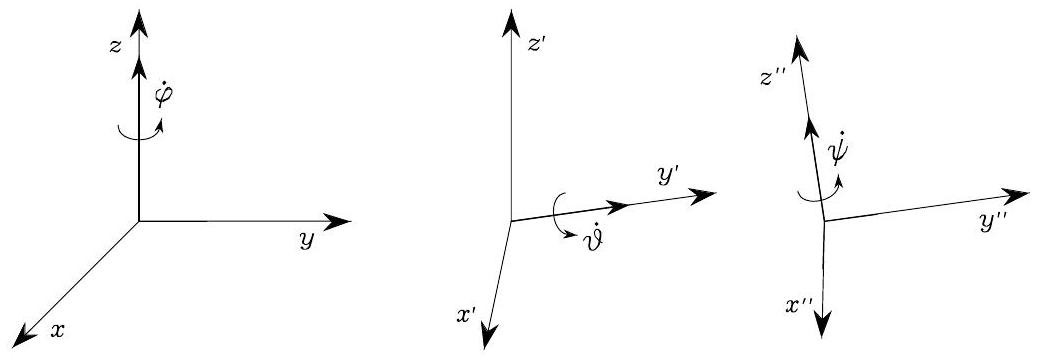
\includegraphics[max width=0.6\textwidth]{diff_kinematics/Euler_angle_vel.jpg}
    \caption{Rotational velocities of Euler angles ZYZ in current frame}
    \label{fig:enter-label}
\end{figure}



\begin{figure}[H]
    \centering
    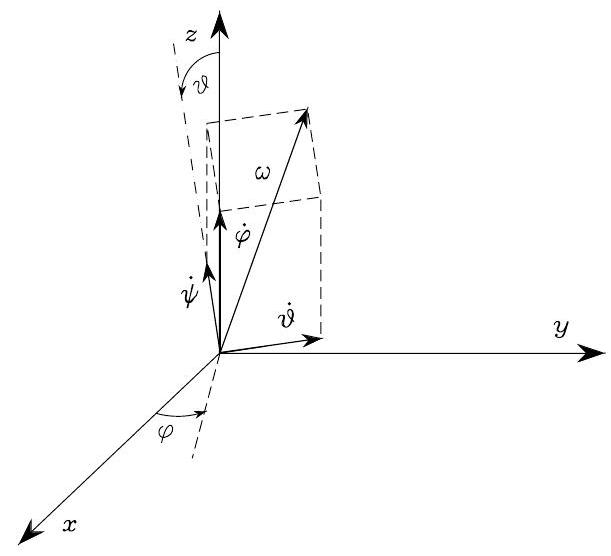
\includegraphics[max width=0.34\textwidth]{diff_kinematics/Euler_angle_vel_to_angular_vel}
    \caption{Composition of elementary rotational velocities for computing angular velocity}
    \label{fig:enter-label}
\end{figure}




The corresponding angular velocity for $\dot{\varphi}$ is $\dot{\varphi}\left[\begin{array}{lll}0 & 0 & 1\end{array}\right]^{T}$

The corresponding angular velocity for   $\dot{\vartheta}$ is  $\dot{\vartheta}\left[\begin{array}{lll}-s_{\varphi} & c_{\varphi} & 0\end{array}\right]^{T}$ 
  
  
The corresponding angular velocity for   $\dot{\psi}$ is   $\dot{\psi}\left[\begin{array}{lll}c_{\varphi} s_{\vartheta} & s_{\varphi} s_{\vartheta} & c_{\vartheta}\end{array}\right]^{T}$,





Thus,

$$
\boldsymbol{T}\left(\phi_{e}\right) =\left[\begin{array}{ccc}
0 & -s_{\varphi} & c_{\varphi} s_{\vartheta} \\
0 & c_{\varphi} & s_{\varphi} s_{\vartheta} \\
1 & 0 & c_{\vartheta}
\end{array}\right] .
$$


\emph{Takeaway:
From a physical viewpoint, the meaning of $\omega_{e}$ is more intuitive than that of $\dot{\boldsymbol{\phi}}_{e}$. The three components of $\boldsymbol{\omega}_{e}$ represent the components of angular velocity with respect to the base frame. Instead, the three elements of $\dot{\phi}_{e}$ represent nonorthogonal components of angular velocity defined with respect to the axes of a frame that varies as the end-effector orientation varies. On the other hand, while the integral of $\dot{\phi}_{e}$ over time gives $\phi_{e}$, the integral of $\omega_{e}$ does not admit a clear physical interpretation, as can be seen in the following example.
}




\end{document}